




 
For a circle centered at $O$, line $\mathcal{L}$ is tangent to this circle at $A$ and has a slope of $-\mathlarger{\frac{1}{2}}$. If the length of $\overline{OB}$ is 2 and $\overline{OB}\perp \overline AB$, then what is the radius of the circle?

 \begin{center}
   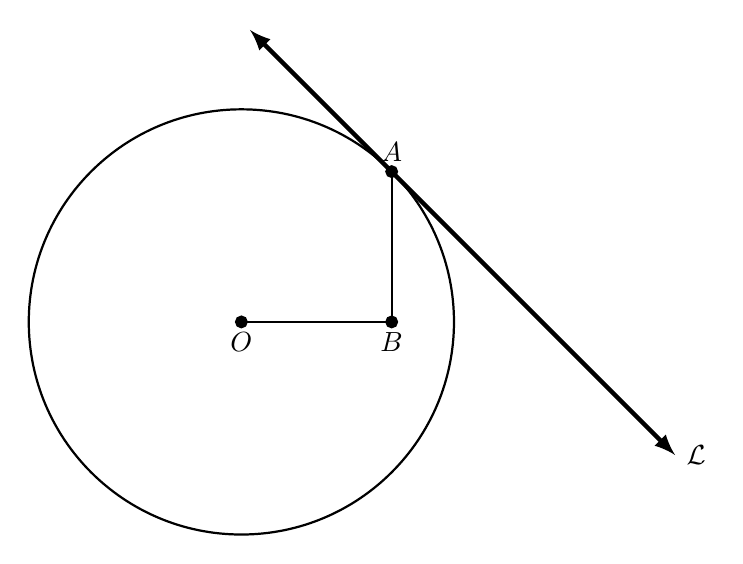
\begin{tikzpicture}[thick,scale=0.9]
     \draw[fill=white] (0,0) circle (3);
\draw[-,thick](0,0)--(.707*3,0)--(.707*3,.707*3);     
\draw[-,thick] (.707*3,0)--(.707*3,.707*3);     
\draw[<->,ultra thick,>=latex](.707*3-2,.707*3+2)--(.707*3+4,.707*3-4) node[right, sloped]{$\mathcal{L}$};
               \draw[fill=black] (0,0) circle (.75mm) node[below]{$O$};
                                     \draw[fill=black] (.707*3,0) circle (.75mm) node[below]{$B$};
                                     
                                                \draw[fill=black] (.707*3,.707*3) circle (.75mm) node[above]{$A$};
 
     
     
   \end{tikzpicture}
 \end{center}


\ifsat
	\begin{enumerate}[label=\Alph*)]
		\item  $2$
		\item  $3\sqrt{2}$
		\item  $2\sqrt{5}$ %
		\item  $6$
	\end{enumerate}
\else
\fi

\ifacteven
	\begin{enumerate}[label=\textbf{\Alph*.},itemsep=\fill,align=left]
		\setcounter{enumii}{5}
		\item  $2$
		\item  $3\sqrt{2}$
		\item  $2\sqrt{5}$ %
		\addtocounter{enumii}{1}
		\item  $4$
		\item  $6$
	\end{enumerate}
\else
\fi

\ifactodd
	\begin{enumerate}[label=\textbf{\Alph*.},itemsep=\fill,align=left]
		\item  $2$
		\item  $3\sqrt{2}$
		\item  $2\sqrt{5}$ %
		\item  $4$
		\item  $6$
	\end{enumerate}
\else
\fi

\ifgridin
  $2\sqrt{5}$ %
		
\else
\fi

